\section{Experimental Design}\label{sec:experiment}

For this case study, the data set to be used is provided by the Faculty of Applied Engineering and Faculty of Science of the University of Antwerp. The data consists of the exam information for the January and June exam period of 2021 and the actual schedule used. For some of the exams, students are split into different groups. This can happen because of room capacity or time constraints. We define for each group of students its own exam to be scheduled. Since these group divisions might not be optimal, further improvements can be made by adding the requirement to split large sets of students into smaller groups when needed.

Even though the two faculties compose their own schedules, the problems are not independent. A section of the rooms are available for both faculties. As a consequence, the schedule has to be generated together. Otherwise a shared exam room could be double booked. The statistics for the data sets provided can be seen in Table \ref{tab:data_set_sem1} and \ref{tab:data_set_sem2}. The fact that the scheduling problem for the Faculty of Applied Engineering and Faculty of Science is not independent can be seen here as well. The statistics for both faculties combined do not equal the sum for the statistics of the faculties separated. The amount of time slots can be calculated as follows:
\begin{equation}
    \text{\# of time slots} = \text{\# Rooms} \times \text{\# Periods} \times \text{\# Exam times}  
\end{equation}
with there being two exam times, namely a morning and afternoon exam. For the January and June schedule, there are respectively 20 and 24 periods.
\begin{table}[H]
	\caption{Data set statistics for January 2021}
	\label{tab:data_set_sem1}
	\centering
	\begin{tabular}{l c c c }
		\hline
		& \textbf{Faculty of Applied Engineering} & \textbf{Faculty of Science} & \textbf{Combined} \\ \hline
		Students & 770 & 1041 & 1811 \\
		Exams & 185 & 360 & 536 \\
	    Rooms & 15 & 45 & 54 \\
        Time slots & 600 & 1800 & 2160 \\ \hline
	\end{tabular}
\end{table}

\begin{table}[H]
	\caption{Data set statistics for June 2021}
	\label{tab:data_set_sem2}
	\centering
	\begin{tabular}{l c c c }
		\hline
		& \textbf{Faculty of Applied Engineering} & \textbf{Faculty of Science} & \textbf{Combined} \\ \hline
		Students & 782 & 1071 & 1852 \\
		Exams & 169 & 342 & 491 \\
	    Rooms & 15 & 45 & 54 \\
        Time slots & 720 & 2160 & 2592 \\ \hline
	\end{tabular}
\end{table}

Tables \ref{tab:workload_sem1} and \ref{tab:workload_sem2} show the workload of students for both data sets. The higher the amount of exams per student, the harder it becomes to create good timetables for students. 


\begin{table}[H]
	\caption{Student workload statistics for January 2021}
	\label{tab:workload_sem1}
	\centering
	\begin{tabular}{l c c c }
		\hline
		\textbf{\# exams per student}& \textbf{Faculty of Applied Engineering} & \textbf{Faculty of Science} & \textbf{Combined} \\ \hline
		Average  & 6.2 & 5.4 & 5.8 \\
		Median & 7 & 6 & 6 \\
	    Max & 11 & 11 & 11 \\
	\end{tabular}
\end{table}

\begin{table}[H]
	\caption{Student workload statistics for June 2021}
	\label{tab:workload_sem2}
	\centering
	\begin{tabular}{l c c c }
		\hline
		\textbf{\# exams per student}& \textbf{Faculty of Applied Engineering} & \textbf{Faculty of Science} & \textbf{Combined} \\ \hline
		Average  & 5.5 & 4.6 & 5.0 \\
		Median & 6 & 5 & 5 \\
	    Max & 10 & 11 & 11 \\
	\end{tabular}
\end{table}

Additionally, we compare the size and student workload statistics of the provided data set with the Toronto benchmark \cite{ceschia2022} (see Section \ref{benchmarks}). This comparison can be seen in Table \ref{tab:workload_compared}. W(avg) and W(max) detail the workload per student. These values, respectively, calculate the average and max amount of exams for every student. This shows that the size of the used data sets is competitive compared to the Toronto benchmark, especially when taking the workload into account.

\begin{table}[H]
	\caption{Student workload statistics compared between different data sets}
	\label{tab:workload_compared}
	\centering
	\begin{tabular}{l c c c c}
		\hline
		\textbf{Data set}& \textbf{Exams} & \textbf{Students} & \textbf{W(avg)} & \textbf{W(max)} \\ \hline
            \textbf{University of Antwerp} \\  \hline
		January 2021  & 536 & 1811 & 5.8 & 11 \\
		June 2021 & 491 & 1852 & 5.0 & 11 \\ \hline
              \textbf{Toronto benchmark instances} \\  \hline
		car91  & 678 & 16925 & 4.2 & 9 \\
		ear83 & 190 & 1125 & 7.2 & 7 \\
            hec92 & 81 & 2502 & 4.3 & 7 \\
            lse91 & 379 & 2627 & 4.2 & 8 \\
            rye93 & 485 & 9458 & 4.8 & 10 \\
            ute92 & 184 & 2672 & 4.4 & 6 \\
            yor83  & 81 & 940 & 6.42 & 14 \\ \hline
	\end{tabular}
\end{table}

In order to compare solutions, we propose the use of both qualitative and quantitative data. In section \ref{qualitative}, we discuss the use of qualitative data based on feedback from the university administration. Section \ref{quantitative} proposes several quantitative scoring metrics to be used. Section \ref{initial} discusses variance present in solutions when running the same analysis multiple times. Finally, section \ref{tuning} looks into optimising the hyper parameters used in the algorithm.

All analyses reported in the following subsections were conducted on a personal computer running an Intel Core i7-6700HQ processor with 16GB of RAM memory.

\subsection{Qualitative data} \label{qualitative}

The software used by the university administration is capable of exporting exam timetables into an Excel document. In order to provide the administrators with a familiar format, we export our generated timetables into the same Excel format. Every file corresponds to the entire timetable for one exam period and contains three data sheets, each visualising the timetable in a different manner. The first sheet details for every student the exams in which they are enrolled, and provides information on the scheduled exam such as the exam form (oral, written, PC, etc.), date, time (morning or afternoon), and room. An example for this sheet can be seen in Figure \ref{fig:sheet1}. 

\begin{figure}[H]
	\centering
	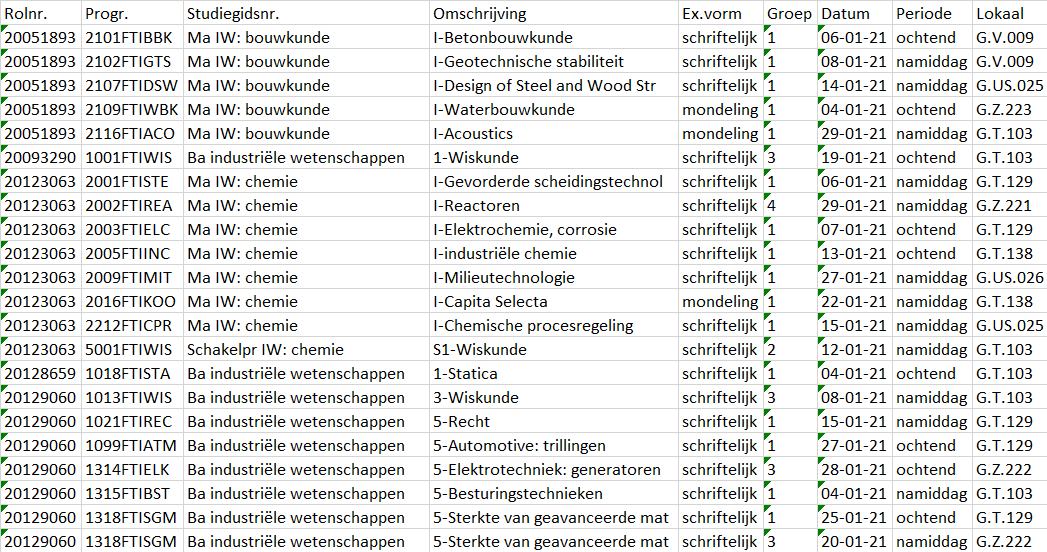
\includegraphics[width=0.7\textwidth]{images/excel/excel_sheet1.png} 
	\caption{Qualitative data: exam details per student}
	\label{fig:sheet1}
\end{figure}

The second sheet, shown in Figure \ref{fig:sheet2}, provides for every student the timetable of their study programmes. This is important because students can be enrolled in multiple study programmes. For example, a student can be enrolled in both an undergraduate and graduate degree when they are not enrolled in the model track. A student having more than one exam on the same day is visualised by a red block, highlighting the constraint violation.

\begin{figure}[H]
	\centering
	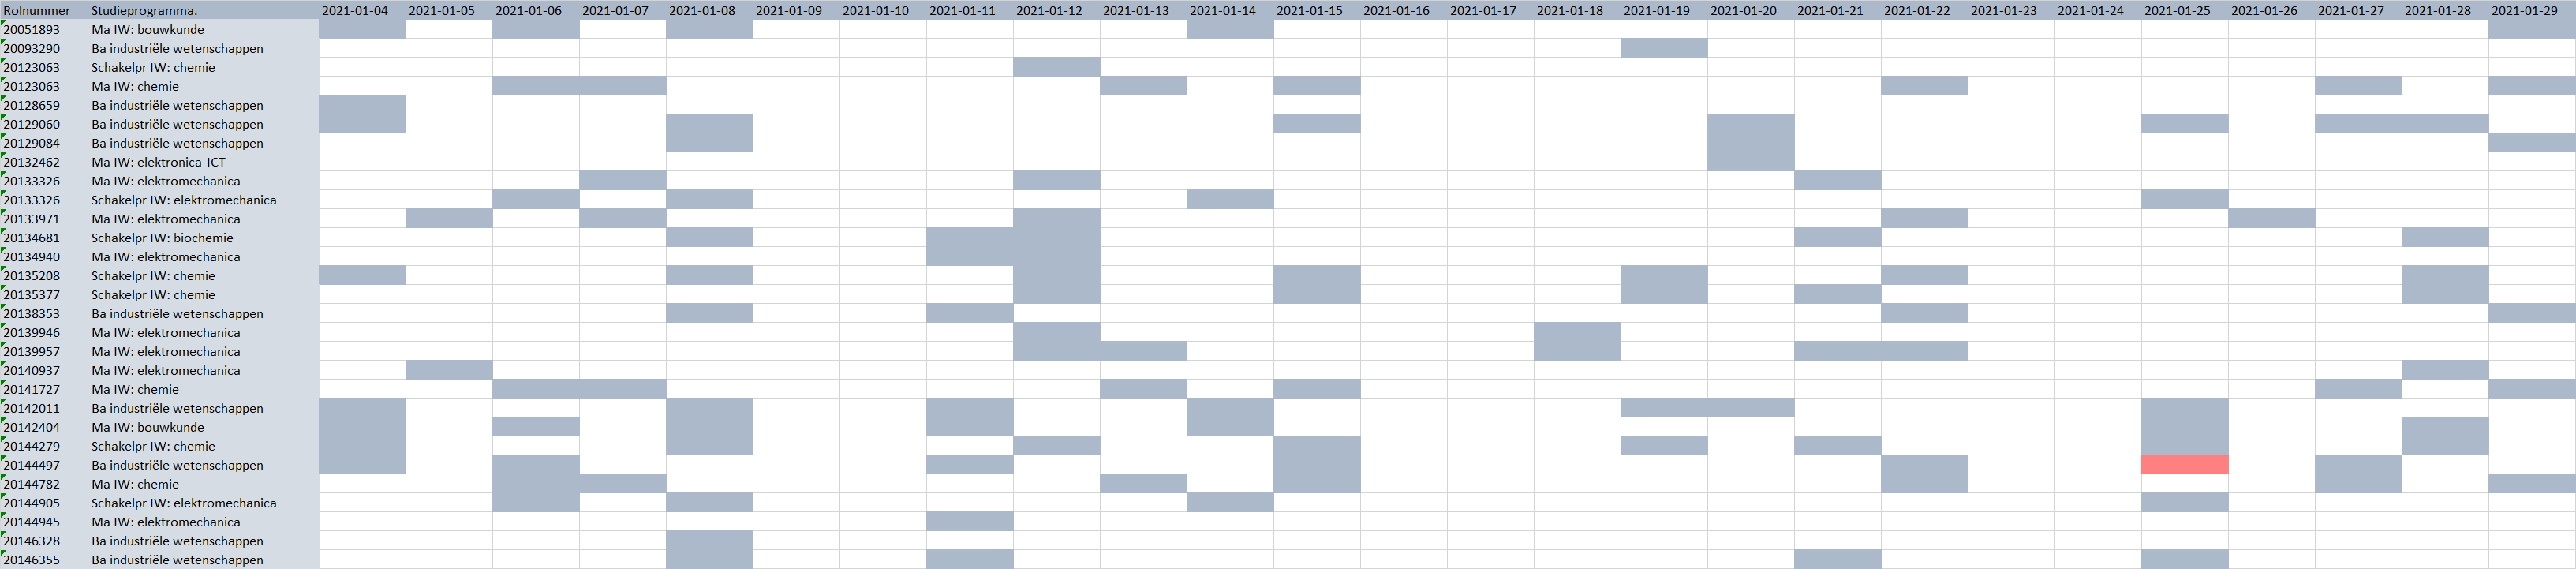
\includegraphics[width=0.9\textwidth]{images/excel/excel_sheet2.png} 
	\caption{Qualitative data: exam schedule per study programme}
	\label{fig:sheet2}
\end{figure}

The last sheet, shown in Figure \ref{fig:sheet3}, visualises for every student the overall timetable and the different exams. This provides an overview of all students their timetables. Additionally, it makes it possible to quickly identify which exams are conflicting for a student.

\begin{figure}[H]
	\centering
	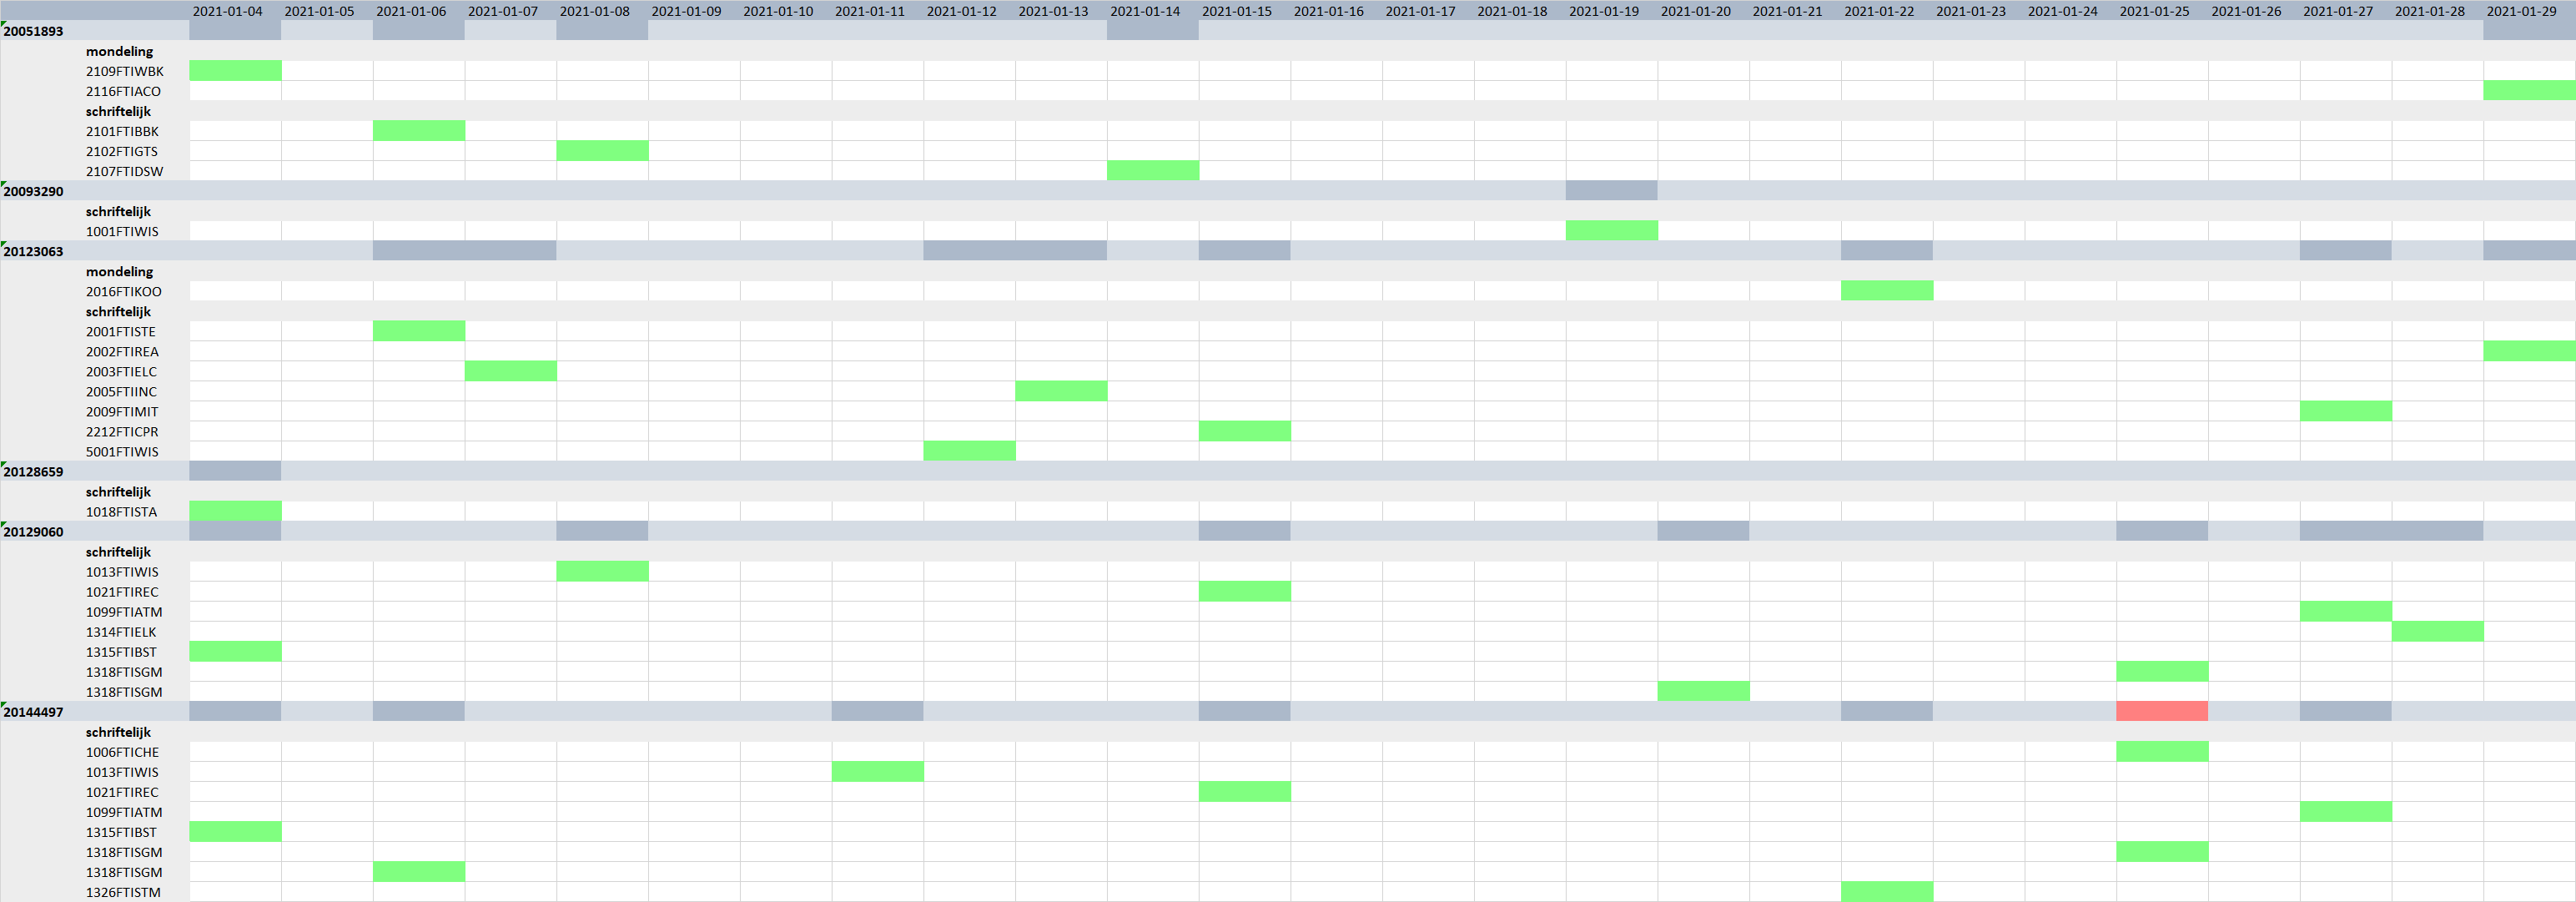
\includegraphics[width=0.9\textwidth]{images/excel/excel_sheet3.png} 
	\caption{Qualitative data: exam schedule per student}
	\label{fig:sheet3}
\end{figure}

\subsection{Quantitative data} \label{quantitative}

The size of university timetabling schedules can make it hard to visually evaluate generated solutions. In order to objectively and consistently evaluate these solutions, we use several quantitative scoring metrics that can be used to compare and rank solutions.

First, the objective function is used in most research to compare solutions. Additionally, it is already used during the search to compare neighbours. This provides a consistent metric to rank solutions generated by both the algorithm and the university administration. However, this objective value does not allow to intuitively explain the quality of the solution. Additionally, having a second scoring metric will be required when trying to optimise the objective function. Since changing the weights of the function has an impact on its value, an independent measure is needed.

Thus, the average time between exams was considered as a timetable benchmark. However, this does not provide a suitable metric as the average can be easily skewed by outliers such as students having a low amount of exams. Instead the actual distribution of time between exams can be used. The importance of this metric became clear from the feedback provided by the university administrators. More notable, we use the percentage of times that students have exam conflicts, have 1 day between exams, 2 days, and finally 3+ days. While this does not result in a single metric, it allows for a good indication of the quality. This is because the administration attempts to provide at least 2 days between exams for the model track, and preferably 3 or more.

\subsection{Variance in results} \label{initial}

In order to compare results between different runs, we must first look at how much variance there is when running the same analysis multiple times. We look at the impact the initial solution has on the optimisation phase and the final solution. As explained in Section \ref{initialisation}, the initial solution takes all hard constraints into account except the exam conflicts between solutions. However, every exam is assigned a random time slot as long as its room type and capacity meet the requirements.

Table \ref{fig:multiple_runs} shows the objective function for different analysis runs of version 2 with an identical set of hyper parameters. While there is some variance present, the amount of spread remains limited. Additionally, the impact on the exam distribution can be seen in Table \ref{tab:multiple_runs}. Even though some differences in distribution are visible, the standard deviation remains low. This makes that the results of our analyses can be considered robust, meaning the majority of duplicate runs will be very similar. Nonetheless, for all comparisons, we will select the best run out of several in order to provide the most accurate comparison.

\begin{figure}[H]
	\centering
	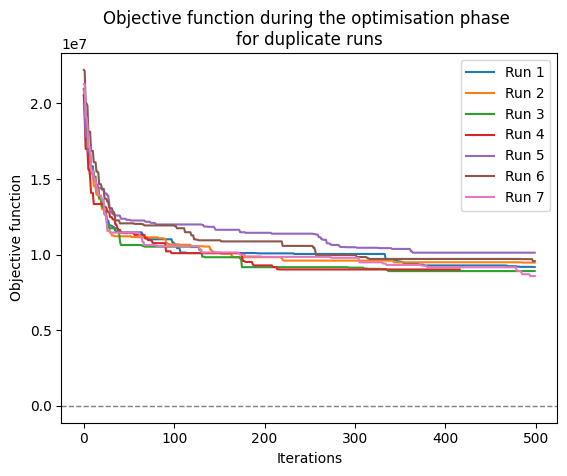
\includegraphics[width=0.75\textwidth]{images/initial/multiple_runs.png} 
	\caption{Objective function when running the same analysis multiple times}
	\label{fig:multiple_runs}
\end{figure}

\begin{table}[h]
	\caption{Exam distribution between duplicate runs}
	\label{tab:multiple_runs}
	\centering
	\begin{tabular}{c c c c c c}
		\hline
  	\textbf{Run}	&
   \textbf{0 days \% } &
    \textbf{1 day \% } & 
    \textbf{2 days \% } &
    \textbf{3 days \% } & 
    \textbf{4+ days \%}\\ \hline
    Run 1 & 0.1\% & 8.4\% & 8.5\% & 22.5\% & 60.5\% \\
    Run 2 & 0.0\% & 8.6\% & 9.1\% & 20.3\% & 62.0\% \\
    Run 3 & 0.0\% & 8.0\% & 8.7\% & 22.3\% & 61.0\% \\
    Run 4 & 0.0\% & 9.2\% & 7.1\% & 23.1\% & 60.6\% \\
    Run 5& 0.0\% & 9.2\% & 9.7\% & 20.9\% & 60.2\% \\
    Run 6 & 0.0\% & 8.0\% & 7.4\% & 22.6\% & 62.0\% \\ \hline
    
    Average& 0.0\% & 8.6\% & 8.4\% & 22.0\% & 61.1\%\\
    Median & 0.0\% & 8.6\% & 8.6\% & 22.4\% & 60.8\% \\\hline
    
    Standard Deviation & 0.0\% & 0.5\% & 1.0\% & 1.1\% & 0.78\%\\
        \hline
	\end{tabular}
\end{table}

\subsection{Parameter tuning} \label{tuning}

Parameter tuning is important in order to optimise the performance of search methods. The different hyper parameters  available for the algorithm versions can be seen in Table \ref{tab:possible_parameters}. With MAX\_ITER\_OPTIMISATION and MAX\_ITER\_INITIALISATION defining the duration of the algorithm run time, the main variables to set are the weights. Unlike P\_INITIALISATION being a single value, P\_OPTIMISATION is a list with the value at index $i$ corresponding to the penalty for two exams at distance $i$. If there is no value at index $i$, the penalty is equal to 0.

\begin{table}[h]
	\caption{Tabu search hyper parameters}
	\label{tab:possible_parameters}
	\centering
	\begin{tabular}{l c c}
		\hline
		& \textbf{Parameter} & \textbf{Description}  \\ \hline
        \textbf{All versions} & &\\ 
		& P\_INITIALISATION & weight of conflicts during initialisation phase \\
        & P\_OPTIMISATION  & weight of distance between exams\\
	    & MAX\_ITER\_INITIALISATION & max amount of iterations during initialisation phase \\
        & MAX\_ITER\_OPTIMISATION & max amount of iterations during optimisation phase\\ 
        & TABU\_LIST\_SIZE & size of the tabu list used\\
        \textbf{Version 3} & &\\ 
        & MAX\_MOVES & amount of moves to evaluate each iteration \\ 
        \hline
	\end{tabular}
\end{table}





\subsubsection{TABU\_LIST\_SIZE }

The TABU\_LIST\_SIZE hyper parameter is partly responsible for determining the balance between exploration and exploitation by blocking previously used moves to be applied. Larger tabu lists encourage exploration, which aids the search in escaping local optima. However, if the size is too large, the amount of exploitation is minimised and promising solutions may not be further optimised. Hence, the tabu list size can be a crucial component in the search's performance.

Originally, the size of the tabu list was calculated by Alvarez-Valdes et al. as:

\begin{equation}
    \text{Tabu list size} = \lfloor \sqrt{\text{\# Exams} * \text{\# Periods}}\rfloor
\end{equation}

In order to tune the size of the tabu list (Equation \ref{eq:list}), we add a weight $w$ to it, resulting in:

\begin{equation}
    \text{Tabu list size} = \lfloor\text{w} * \sqrt{\text{\# Exams} * \text{\# Periods}}\rfloor
\end{equation}

By having the weight either smaller or larger than 1, we can perform an analysis with a smaller or larger tabu list size. For the tuning, the weights $w$ were set to 0.1, 0.25, 0.5, 0.75, 1, 2, and 3, resulting in tabu list sizes of 6, 15, 31, 47, 63, 126, and 189, respectively. The impact on the objective by changing the tabu list size can be seen in both Figure \ref{fig:tuning_tabu} and Table \ref{tab:tuning_tabu_obj}. Based on the objective function, using a weight of 0.5  has the most positive impact on the objective of the solutions. This means that the tabu list size to be used is half of the proposed size by Alvarez-Valdes et al. Table \ref{tab:tuning_tabu_distr} explains this decrease in objective by showing a lower amount of occurrences where a student has only 1 day between exams compared to the other results. Every 'x days \%' column indicates the percentage of occurrences where a student has x days between exams. 

\begin{figure}[H]
	\centering
	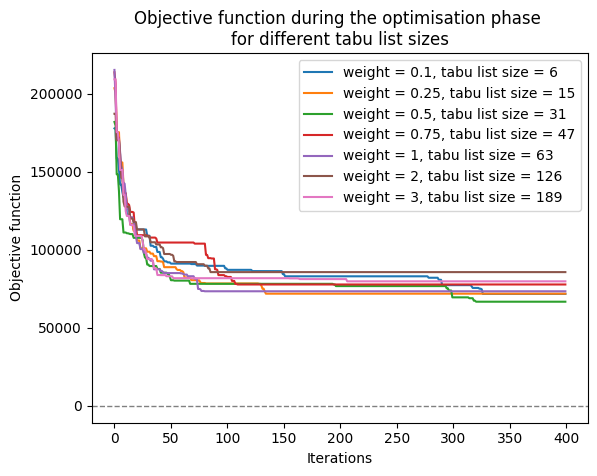
\includegraphics[width=0.75\textwidth]{images/tuning/tabu_list.png} 
	\caption{Objective function when testing different TABU\_LIST\_SIZE \\ values for the Faculty of Science June data set}
	\label{fig:tuning_tabu}
\end{figure}

\begin{table}[h]
	\caption{Effect of tabu list size on objective functions}
	\label{tab:tuning_tabu_obj}
	\centering
	\begin{tabular}{l c c c }
		\hline
  	\textbf{Weight $w$}	                & 
     	\textbf{Tabu list size}	                & 
    \textbf{Objective} & 
    \textbf{Objective difference vs $w$ = 1} \\ \hline
        0.1 & 6 & 71738 & -2.3\%  \\ 
        0.25& 15 & 71908 & -2.1\%  \\ 
        0.50 & 31 & 66764 & -9.1\%  \\ 
        0.75 & 47 & 77798 & 5.9\% \\
        1 & 63 &73450 & 0.0\% \\
        2 & 126 & 85728 & 16.7\% \\
        3 & 189 & 79824 & 8.7\% \\
        \hline
	\end{tabular}
\end{table}

\begin{table}[h]
	\caption{Effect of tabu list size on exam distribution}
	\label{tab:tuning_tabu_distr}
	\centering
	\begin{tabular}{c c c c c c c}
		\hline
  	\textbf{Weight $w$}	&
   \textbf{Tabu list size} &
   \textbf{0 days \% } &
    \textbf{1 day \% } & 
    \textbf{2 days \% } &
    \textbf{3 days \% } & 
    \textbf{4+ days \%}\\ \hline
    0.1 & 6 & 0.0\% & 6.2\% & 11.0\% & 19.5\% & 63.3\% \\
    0.25 & 15 & 0.0\% & 6.1\% & 10.6\% & 20.3\% & 63.0\% \\
    0.5 & 31 & 0.0\% & 5.0\% & 12.8\% & 21.3\% & 60.9\% \\
    0.75 & 47 & 0.0\% & 6.7\% & 12.8\% & 21.4\% & 59.1\% \\
    1 & 63 & 0.0\% & 6.0\% & 14.0\% & 14.0\% & 66.0\% \\
    2 &  126 & 0.0\% & 8.3\% & 14.2\% & 20.2\% & 57.3\% \\
    3 &  189 & 0.0\% & 6.7\% & 12.7\% & 24.8\% & 55.8\% \\
        \hline
	\end{tabular}
\end{table}

\subsubsection{P\_INITIALISATION \& P\_OPTIMISATION}

Since the initialisation phase is successful in obtaining feasible timetables (Section \ref{phase_init}), we do not further explore fine tuning P\_INITIALISATION. The optimisation phase is responsible for improving the distribution to result in a more optimal timetable. Because of this, we look into tuning the P\_OPTIMISATION weights.

For P\_OPTIMISATION, we look at the results from four sets of weights. Every weight $w_x$ penalises exams with $x$ days between the two exams. If no weight is present for $w_x$, the weight is set to 0.  First, we test the set of weights described by Alvarez-Valdes et al. namely $w_0$ = 3000, $w_1$ = 100, $w_2$ = 20, $w_0$ = 5, $w_4$ = 3, and $w_5$ = 1. Second, the weights 16, 8, 4, 2, and 1 are used for the Carter benchmarks \cite{carter1996}. Finally, we add two sets of weights that have a higher penalty for $w_1$ and $w_2$ than the one for $w_0$ in order to force the distribution to change after the initialisation phase. The weights used for this are [100, 5000, 2000, 50, 30, 5] and [250, 3000, 1000, 50, 30, 5]. Since a change in weights will impact the objective function, the exam distribution has to be used in order to determine the best set of weights.

\begin{table}[h]
	\caption{Effect of objective weights on exam distribution}
	\label{tab:weights_distr}
	\centering
	\begin{tabular}{c c c c c c}
		\hline
  	\textbf{Weights $w_x$}	&
   \textbf{0 days \% } &
    \textbf{1 day \% } & 
    \textbf{2 days \% } &
    \textbf{3 days \% } & 
    \textbf{4+ days \%}\\ \hline
    3000, 100, 20, 5, 3, 1 & 0.0\% &  8.8\% & 12.3\% & 18.1\% & 60.8\% \\
    16, 8, 4, 2, 1 & 0.0\% & 7.4\% & 13.7\% & 18.3\% & 60.6\% \\
    100, 5000, 2000, 50, 30, 5 & 0.0\% & 7.6\% & 9.6\% & 20.2\% & 62.6\% \\
    250, 3000, 1000, 50, 30, 5 & 0.0\% &  7.9\% & 11.9\% & 19.3\% & 60.9\% \\
        \hline%
	\end{tabular}
\end{table}

Table \ref{tab:weights_distr} shows the resulting distribution after a maximum of 1000 iterations (fewer if no improved solution has been found after 200 iterations). While the weights of the Carter benchmark (16, 8, 4, 2, and 1) provide the lowest amount of exams occurrences with a single day between them, the third set of weights provides a better overall distribution. Even though it has a slightly higher percentage of occurrences for exams at distance 1, it significantly lowers the amount of exams at a distance of 2 days compared to the other weights.


\subsubsection{MAX\_ITER\_OPTIMISATION \& MAX\_MOVES}

Thompson and Dowsland \cite{thompson1996} showcase that longer searches are able to generate better solutions. This can be explained by a longer search resulting in more solutions being visited in the search space. This results in a larger possibility of encountering good solutions. The hyper parameters MAX\_ITER\_OPTIMISATION \& MAX\_MOVES both impact the duration of the search. While MAX\_ITER\_OPTIMISATION increases the amount of iterations for the search to end, MAX\_MOVES increases the amount of time spent on each iteration. 

Previous analyses have shown that the search is generally able to converge in fewer than 500 iterations to the point where no improvement is found for at least 200 iterations. This is visible in Figure \ref{fig:tuning_tabu} where all runs end with a flat lining objective function. While better solutions may still be found due to the search currently being stuck in a local optimum, terminating the solution after a cut off point is considered acceptable. Because of this, the importance of having a high value for MAX\_ITER\_OPTIMISATION is reduced.

The impact of increasing the MAX\_MOVES parameter is tested on both the execution time and objective function. The values tested for MAX\_MOVES are 250, 500, 750, 1000, and 1500. Figure \ref{fig:tuning_execution} shows that increasing MAX\_MOVES generally also lowers the objective function. 

\begin{figure}[H]
	\centering
	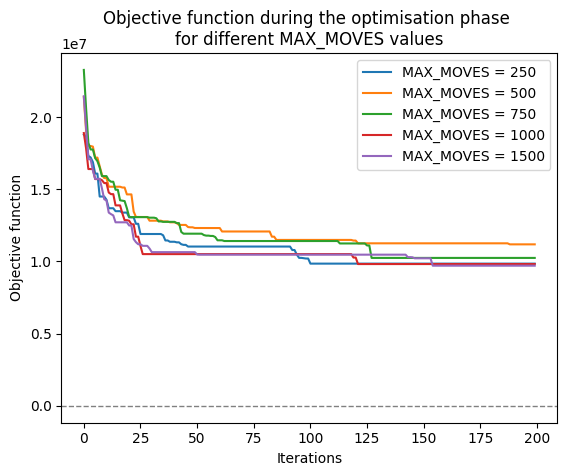
\includegraphics[width=0.75\textwidth]{images/tuning/max_moves_objective.png} 
	\caption{Objective function when testing different MAX\_MOVES \\ values for the combined June data set}
	\label{fig:tuning_objective}
\end{figure}

Additionally, Figure \ref{fig:tuning_execution} visualises the relation of the value for MAX\_MOVES and the execution time. It shows that increasing MAX\_MOVES also results in a longer execution time per iteration. Since a MAX\_MOVES value of 250 results in one of the best objective function at the lowest time penalty, we will use this value for further analyses. 

\begin{figure}[H]
	\centering
	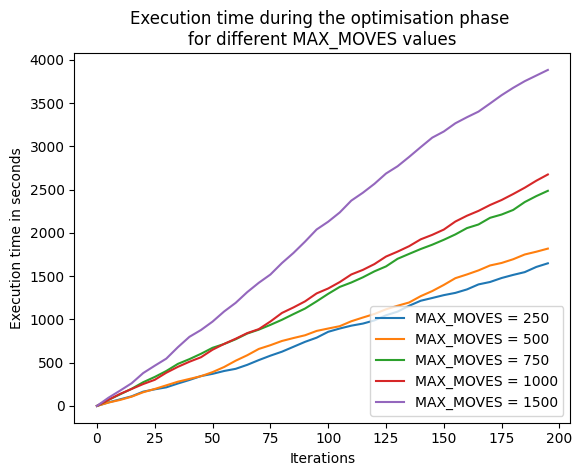
\includegraphics[width=0.75\textwidth]{images/tuning/max_moves_execution.png} 
	\caption{Execution time when testing different MAX\_MOVES \\values for the combined June data set}
	\label{fig:tuning_execution}
\end{figure}
